\chapter{密码学概论}
\question{密码学分支}
\begin{enumerate}
	\item 密码编码学,将明文转换为密文
	\item 密码分析学,破译密文
\end{enumerate}

\question{密码元素}
\begin{enumerate}
	\item 明文
	\item 密文
	\item 加密
	\item 解密
	\item 密钥
\end{enumerate}
\textbf{三元素:}明文,密钥,密文\\
\textbf{五元素:}明文空间、密文空间、密钥空间、加密算法、解密算法。

\question{密码分析方法}
\begin{enumerate}
	\item 唯密文攻击:密码分析者拥有一些消息的密文,这些消息都是用同样的加密算法来加密的
	\item 已知明文攻击:密码分析者不仅拥有一些消息的密文,而且还拥有这些密文对应的明文
	\item 选择明文攻击:分析者不仅拥有一些消息的密文和相应的明文,而且他们还可以进行有选择地加密明文。
	\item 选择密文攻击:密码分析者能够选择不同的密文,而且能够得到与之对应的明文。
\end{enumerate}

\indent \textbf{攻击强度递增},唯密文是最弱的一种攻击,选择密文是最强的一种攻击,如果一个系统能够抵抗选择密文攻击,他一定能够抵抗其他攻击。\\

衡量密码攻击的复杂度有两个方面:
\begin{itemize}
	\item 数据复杂度,为了实施攻击所需输入的数据量
	\item 处理复杂度,处理这些数据所需的计算量
\end{itemize}


\question{凯撒算法}
\begin{gather}
C=E(p)=(p+k) mod 26 \\ 
p=D(C)=(C-k) mod 26
\end{gather}
\question{维吉尼亚加密算法}
生成维吉尼亚矩阵,和\textbf{与明文长度一样的密钥},然后明文找列,密钥找行,生成密文。
\begin{figure}[H]
	\centering
	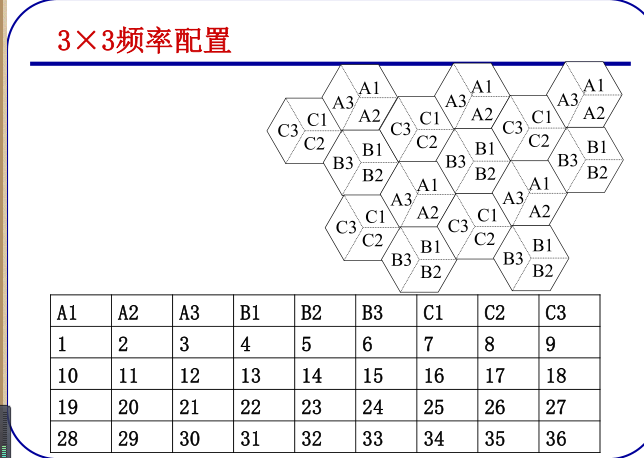
\includegraphics[width=0.7\linewidth]{screenshot006.png}
\end{figure}

\question{现代加密算法分类}
\begin{enumerate}
	\item 对称加密算法,加解密都采用一样的密钥,加/解密速度快,但密钥分发问题严重
	\item 非对称加密算法,加解密采用不同密钥,加/解密速度较慢,但无密钥分发问题
\end{enumerate}

\question{DES} 是一种\textbf{块加密算法},\textbf{对称加密算法},每块64bit。
\begin{figure}[H]
	\centering
	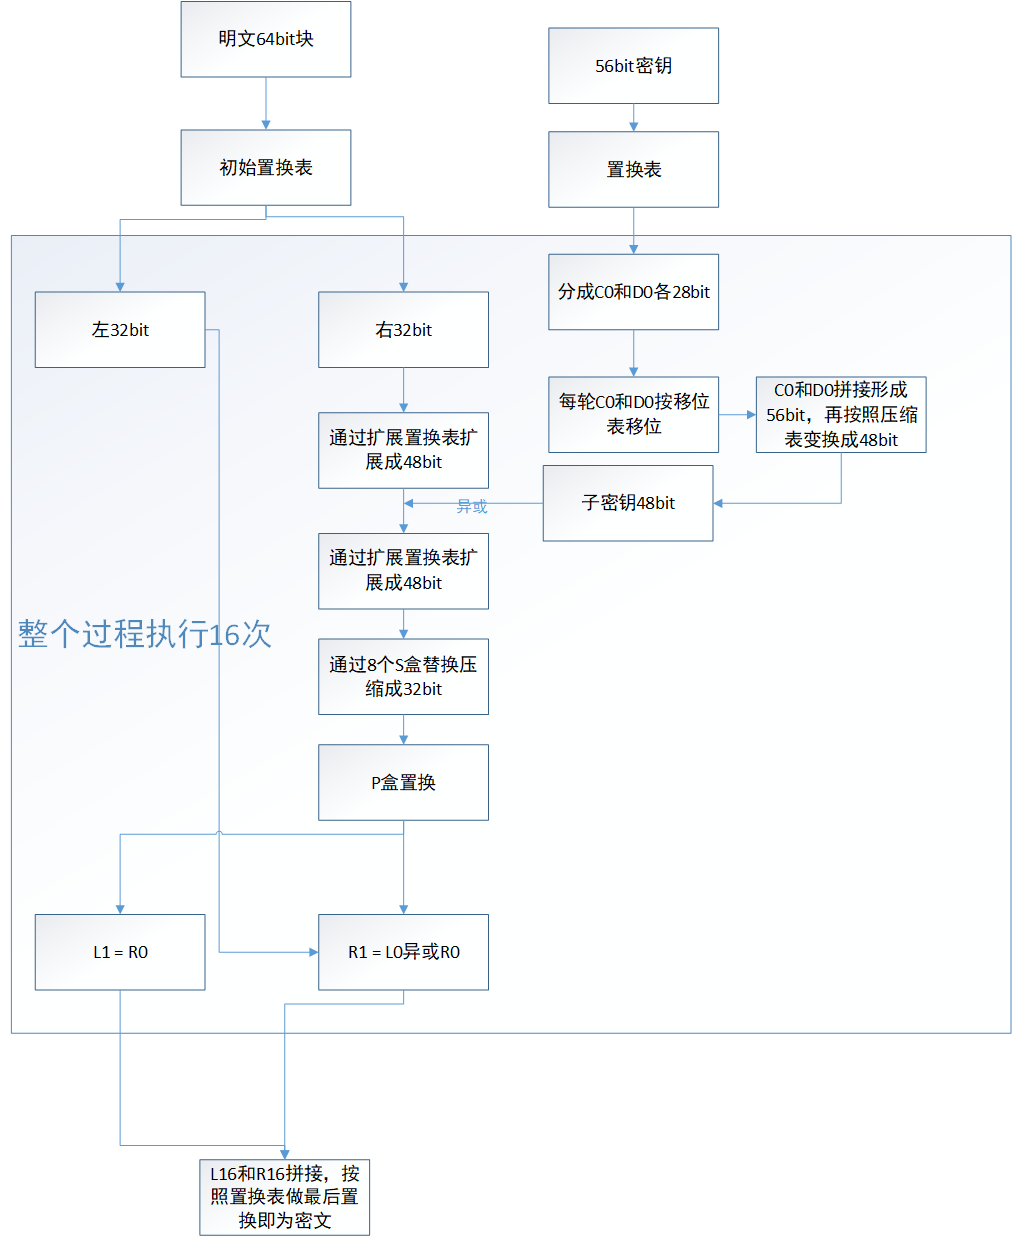
\includegraphics[width=0.7\linewidth]{figures/screenshot007}
	\caption{}
	\label{fig:screenshot007}
\end{figure}

\question{其余几种对称加密算法}
\begin{enumerate}
	\item IDEA,64位输入,128位密钥,64位输出
	\item AES ,128bit输入,密钥长度可变,为 128/192/256bit,相应的轮数 r为 10/12/14
	\item 2DES,采用两个密钥(不相同),加密时,先使用$ K_2 $加密,再使用$ K_1 $加密,解密时先使用$ K_1 $解,在使用$ K_2 $解
	\item 3DES.重复三次。
\end{enumerate}

\question{RSA算法} 非对称加密算法,安全性基于分解大整数的困难性\\
公钥与密钥的产生
\begin{enumerate}
	\item 随意选择两个大的质数p和q,p不等于q,计算N=pq。
	\item 根据欧拉函数,求得r = (p-1)(q-1)
	\item 选择一个小于 r 的整数 e,求得 e 关于模 r 的模反元素,命名为d。(模反元素存在,\textbf{当且仅当e与r互质})
	\begin{equation}\label{key}
	e\times d = 1\ mod\ r
	\end{equation}
	\item 将 p 和 q 的记录销毁。
\end{enumerate}
(N,e)为公钥,(N,d)为私钥。\textbf{采用公钥加密,私钥解密}\\
一个实例
\begin{gather}
 p = 3,q=11 , N = pq = 33\\
 r = (p-1)(q-1) = 2*10 = 20 \\
 ed = r * n + 1\\
 e = 3,d = 7\\
\end{gather}
所以公钥(33,3),私钥(33,7)。要传输的消息m = 24
\begin{gather}
 \text{加密}\quad m^e mod N = 24^3 \% 33 = 30\\
 \text{解密}\quad c^d mod N = 30 ^d \% 33 =24
\end{gather}


\question{密钥管理}
\begin{enumerate}
	\item 密钥生成,两方或多方提供共享的秘钥以便在以后的安全通信中进行加密解密、消息认证或身份认证。
	\item 密钥传送,由一方建立密钥,然后安全地传送给其他地方
	\begin{enumerate}
		\item 点对点模式需要共享密钥的双方直接通信,传递密钥,即采用人工分发的形势,也可以通过数字信封,
		用一个双方预先共享的密钥来加密新密钥,然后通过 Internet 传送;
		\item 密钥服务器模式需要密钥服务器(Key Server, KS)
		的参与,分为两种情况:其一,密钥服务器生成密钥,然后通过安全信道分别传送给通信的各方;其二,密钥服务器
		只负责密钥的传递,不负责密钥的生成。密钥的生成由通信各方中的一方生成。
	\end{enumerate}
	\item 密钥协商,双方或多方共同参与密钥形成过程中。通过 DH 密钥交换协议,通信双方能够在不安全的通信信道上传递公开信息,继而各自计算出共享密钥。
\end{enumerate}


